\documentclass[13pt]{article}
\usepackage[utf8]{inputenc}
\usepackage{tikz}
\usetikzlibrary{quantikz}
\usepackage{physics}
\usepackage{pgfplots}
\usepgfplotslibrary{units}
\usetikzlibrary{patterns}
\usepackage{siunitx}
\usetikzlibrary{angles, quotes}
\usepackage{amssymb}
\usetikzlibrary{angles, arrows.meta, quotes}
\pgfplotsset{compat=1.17}

\usepackage{minted}
\usepackage[most]{tcolorbox}
\definecolor{lightgreen}{rgb}{0.56, 0.93, 0.56}
\definecolor{moonstoneblue}{rgb}{0.45, 0.66, 0.76}

\newtcblisting{myminted}{%
    listing engine=minted,
    minted language=c,
    listing only,
    breakable,
    enhanced,
    minted options = {
        linenos,
        breaklines=true,
        breakbefore=.,
        fontsize=\footnotesize,
        numbersep=2mm
    },
    overlay={%
        \begin{tcbclipinterior}
            \fill[gray!25] (frame.south west) rectangle ([xshift=4mm]frame.north west);
        \end{tcbclipinterior}
    }
}

\title{Grover's Algorithm Tutorial/Experimentation}
\author{Rahul Goel}
\date{November 2020}

\begin{document}

\maketitle

\textbf{Note - It has been assumed that $N = 2 ^ n$ throughout this sheet.}

\section{The Problem - Needle in a Haystack}
\indent The problem that Grover's Algorithm solves is the unstructured search problem. In simple words, among $N$ given entities, our task is to find one unique entity that satisfies a particular property.

In most cases, the situation is random and the only way a classical computer knows how to solve it is by brute force. This can take $O(N / 2)$ on average and up to $O(N)$ time in the worst case.

The problem of unstructured search is considered to be a hard problem for a classical computer as $N$ gets bigger in size. Grover's Algorithm provides a quadratic speedup to this and reduces the number of queries (time taken) to $O(\sqrt{N})$. In fact, it has been proven that for a quantum computer, this is the best possible time complexity.

Note - The problem gets easier and the complexity gets reduced by a constant factor when the entities that satisfy the property are more in number.

\section{How the Algorithm works}
\subsection{Intution 1}
Initially, we start with $n$ qubits in such a way that in their superposition, all the $N$ states have equal amplitude (each has an equal probability of popping up when we measure the state).
$$\ket{\psi_{initial}} = \sum_{0}^{N-1} {\alpha_i}\ket{i} \text{ where } \alpha_i = \frac{1} {\sqrt{N}}$$

Let $\ket{j}$ be our needle in the haystack.
Now, by means of certain quantum gates, the amplitude $\alpha_j$ is first negated i.e. it becomes $-\alpha_j$. And then every single $\alpha_i$ is flipped about the mean of all amplitudes. As a result, $\alpha_j$ stands out more than every other $\alpha_i$.
\\[3cm]
\indent This has been explained by means of the following diagrams (Not to scale).
Initially the amplitudes of all the states are equal and the sum of their squares is equal to $1$.

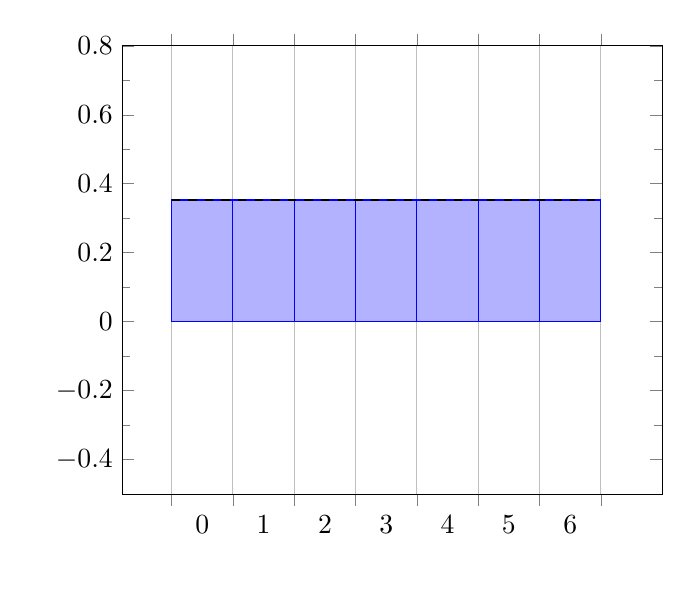
\begin{tikzpicture}
\begin{axis}[ybar interval, ymax=0.8,ymin=-0.5, minor y tick num = 1, xmax = 8]
\addplot coordinates { (0, 0.353) (1, 0.353) (2, 0.353) (3, 0.353) (4, 0.353) (5, 0.353) (6, 0.353) (7,0.353)};
\draw [dashed] (0,0.353) -- (7, 0.353);

\end{axis}
\end{tikzpicture}

Then a quantum circuit is applied to the state which flips the amplitude of the desired state.

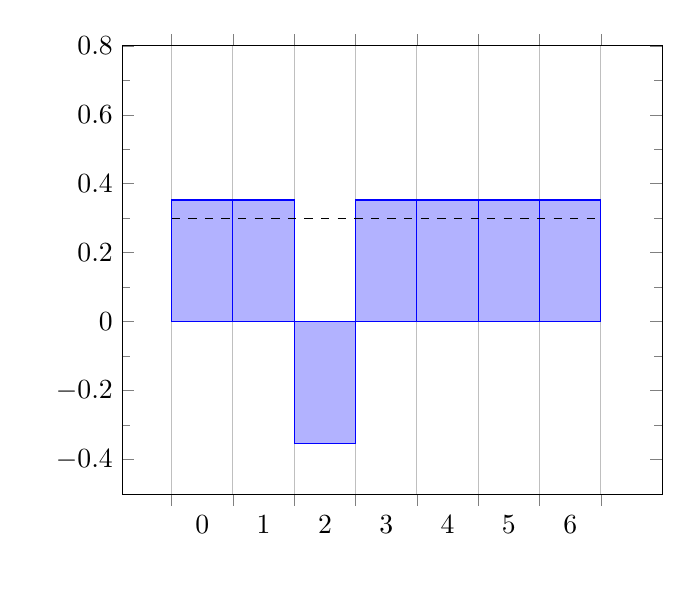
\begin{tikzpicture}
\begin{axis}[ybar interval, ymax=0.8,ymin=-0.5, minor y tick num = 1, xmax = 8]
\addplot coordinates { (0, 0.353) (1, 0.353) (2, -0.353) (3, 0.353) (4, 0.353) (5, 0.353) (6, 0.353) (7,0.353)};
\draw [dashed] (0,0.3) -- (7, 0.3);
\end{axis}
\end{tikzpicture}

Now the inversion of one of the amplitudes results in a slight decrement of the mean of all the amplitudes. If we now flip the amplitudes about their mean, we land up in the following state.

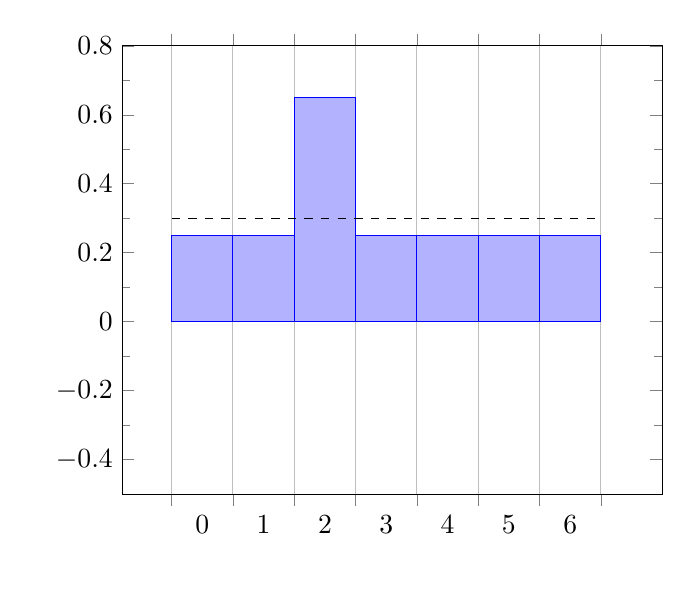
\begin{tikzpicture}
\begin{axis}[ybar interval, ymax=0.8,ymin=-0.5, minor y tick num = 1, xmax = 8]
\addplot coordinates { (0, 0.25) (1, 0.25) (2, 0.65) (3, 0.25) (4, 0.25) (5, 0.25) (6, 0.25) (7,0.25)};
\draw [dashed] (0,0.3) -- (7, 0.3);
\end{axis}
\end{tikzpicture}

The amplitude of the needle in the haystack has increased and hence if we measure the state now, the chance of getting the correct value is more than it was previously. However, the sum of probabilities of getting other states is still greater than the probability of getting the answer.\\[4pt]

Hence, we repeat the negation and inversion steps a number of times so that when we measure the state, we can be pretty sure that the outcome is the answer (the desirable state).\\[4pt]

Initially $\alpha_j = \dfrac{1}{\sqrt{N}}$. As we run iterations of the algorithm, $\alpha_j$ increases and $\alpha_i$, $\forall$ $i \neq j$, decreases, all in such a way that $\sum_0 ^{N-1} {\alpha_i}^2 = 1$.
If we want the probability of getting $\ket{j}$ to be at least half, we need to pump up the magnitude $\alpha_j$ to $\dfrac{1}{\sqrt{2}}$. At the point in time when $\alpha_j = \dfrac{1}{\sqrt{2}}$, $\alpha_i \approx \dfrac{1}{\sqrt{2N}}$ $\forall$ $i \neq j$. Because the amplitude of the other states decreases continuously, we can say that throughout our iterations $\alpha_i \geq \dfrac{1}{\sqrt{2N}}$. Since in one iteration, the amplitude $\alpha_j$ increases by at least by $2 \alpha_i$ $\left( i \neq j\right)$, the increment is at least $\sqrt{\dfrac{2}{N}}$. Therefore the number of iterations required is at least $\dfrac{1 / \sqrt{2}}{\sqrt{2 / N}}$ $=$ $\sqrt{N}$.\\
When the number of favourable states is $M$, the number of iterations comes out to be $\sqrt{\dfrac{N}{M}}$.

\subsection{Intution 2}

Let $\ket{a}$ represent our desirable state i.e. $\ket{j}$. And $\ket{b}$ represent the superposition of all the remaining states with equal amplitudes i.e. $\ket{b} = \sum_{i \neq j} \dfrac{1}{\sqrt{N - 1}} \ket{i}$. It can be easily noticed that $\ket{a}$ and $\ket{b}$ are orthogonal to each other. Let $\psi_0$ be our initial state which is $\sum_{0}^{N - 1} \dfrac{1}{\sqrt{N}} \ket{i}$. Now initially $\ket{\psi_0}$ lies really close to $\ket{b}$ and it is the task of Grover's Algorithm to move it closer to $\ket{a}$.\\[4pt]

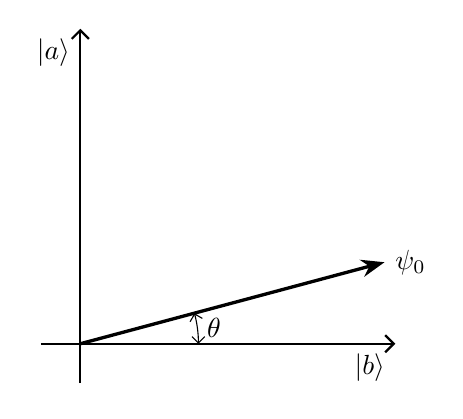
\begin{tikzpicture}[
            > = Straight Barb,
phasor/.style = {very thick,-{Stealth}},
angles/.style = {draw, <->, angle eccentricity=1,
                 right, angle radius=15mm}
                        ]
% coordinates
    \draw[->, thick] (-0.5,0) -- (4,0) coordinate (x) node[below left] {$\ket{b}$};
    \draw[->, thick] (0,-0.5) -- (0,4) node[below left] (y) {$\ket{a}$};
% phasors
    \draw[phasor] (0,0) -- (15:4) coordinate (i)  node[right] {$\psi_0$};% used polar coordinates
% angles drawn by pic
\coordinate (X)   at (0,0);
\draw
    pic["$\theta$",angles] {angle=x--X--i}
    ;
\end{tikzpicture}

The amplitude negation step leads to reflection of $\ket{\psi_0}$ about $\ket{b}$. This is true because $\ket{b}$ represents the superposition of all the undesirable states of equal amplitude. So the projection of $\ket{\psi_0}$ on $\ket{b}$ will remain as it is while the projection of $\ket{\psi_0}$ perpendicular to $\ket{b}$ will get negated. This is nothing but reflection about $\ket{b}$.

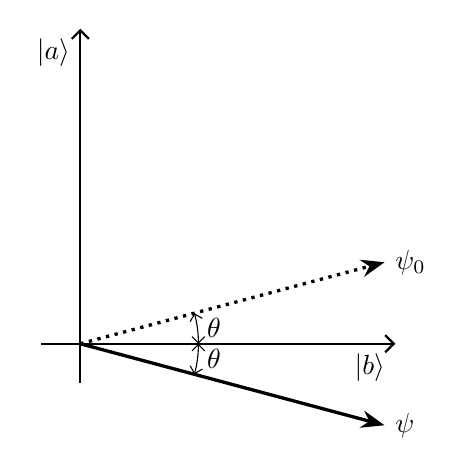
\begin{tikzpicture}[
            > = Straight Barb,
phasor/.style = {very thick,-{Stealth}},
angles/.style = {draw, <->, angle eccentricity=1,
                 right, angle radius=15mm}
                        ]
% coordinates
    \draw[->, thick] (-0.5,0) -- (4,0) coordinate (x) node[below left] {$\ket{b}$};
    \draw[->, thick] (0,-0.5) -- (0,4) node[below left] (y) {$\ket{a}$};
% phasors
    \draw[phasor, dotted] (0,0) -- (15:4) coordinate (i)  node[right] {$\psi_0$};% used polar coordinates
    \draw[phasor] (0,0) -- (-15:4) coordinate (j)  node[right] {$\psi$};% used polar coordinates
% angles drawn by pic
\coordinate (X)   at (0,0);
\draw
    pic["$\theta$",angles] {angle=x--X--i}
    pic["$\theta$",angles] {angle=j--X--x}
    ;
\end{tikzpicture}

Now, we need to do inversion about the mean which is equivalent to reflection about the the equal amplitude state $\sum_{0}^{N - 1} \dfrac{1}{\sqrt{N}} \ket{i}$.

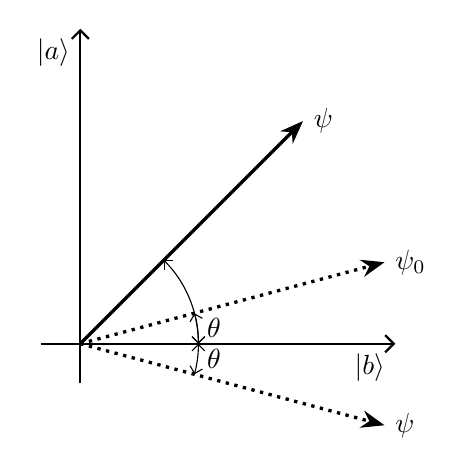
\begin{tikzpicture}[
            > = Straight Barb,
phasor/.style = {very thick,-{Stealth}},
angles/.style = {draw, <->, angle eccentricity=1,
                 right, angle radius=15mm}
                        ]
% coordinates
    \draw[->, thick] (-0.5,0) -- (4,0) coordinate (x) node[below left] {$\ket{b}$};
    \draw[->, thick] (0,-0.5) -- (0,4) node[below left] (y) {$\ket{a}$};
% phasors
    \draw[phasor, dotted] (0,0) -- (15:4) coordinate (i)  node[right] {$\psi_0$};% used polar coordinates
    \draw[phasor, dotted] (0,0) -- (-15:4) coordinate (j)  node[right] {$\psi$};% used polar coordinates
    \draw[phasor] (0,0) -- (45:4) coordinate (k)  node[right] {$\psi$};% used polar coordinates
% angles drawn by pic
\coordinate (X)   at (0,0);
\draw
    pic["$\theta$",angles] {angle=x--X--i}
    pic["$\theta$",angles] {angle=j--X--x}
    pic["",angles] {angle=x--X--k}
;
\end{tikzpicture}

So, after one iteration we have moved closer to the required state. We need to carry these iterations certain number of times so that when we measure a state, it collapses to the desirable state with high probability.

Every time the inversion about mean is done using the equal amplitude state only. It happens to be our initial state too but this is true only for the first iteration and not for further iterations.

\section{How to Implement the circuit?}

Now that we know what to do, we have to question how to do it.
\subsection{Negation of Amplitude}
Our first task is to negate the amplitude of the desirable quantum state.
The situation is like this that we have been given a quantum black box that outputs 1 for the desirable states and 0 for the undesirable states.

Insert diagram here.

In other words, given the superposition $\ket{x}\ket{0}$, the circuit spits out the superposition $\ket{x}\ket{f(x)}$. We know the quantum circuits are designed in such a way that the answer register gets XORed with the output $f(x)$. So if the input superposition is $\ket{x}\ket{y}$, then the output superposition will be $\ket{x}\ket{y \oplus{f(x)}}$.

With this knowledge, we can apply neat little hack and trick our black box into doing the task for us. We will initialise the answer register to $\ket{-}$. Since

\begin{align*}
\ket{-} &= \dfrac{1}{\sqrt{2}} ( \ket{0} - \ket{1} )\\
\ket{- \oplus {f(x)}} &= \dfrac{1}{\sqrt{2}} \left( \ket{0 \oplus {f(x)}} - \ket{0 \oplus {f(x)}} \right)\\
\ket{- \oplus {f(x)}} &= \dfrac{1}{\sqrt{2}} \left( \ket{{f(x)}} - \ket{\overline{f(x)}} \right)\\
\ket{- \oplus {f(x)}} &= \dfrac{1}{\sqrt{2}} \left( -1 \right) ^ {f(x)} \left( \ket{0} - \ket{1} \right)\\
\ket{- \oplus {f(x)}} &= \left( -1 \right) ^ {f(x)} \ket{-}\\
\end{align*}

Therefore, the entire transition will be
$$\ket{x}\ket{-} \longrightarrow \left( -1 \right) ^ {f(x)} \ket{x} \ket{-}$$

Now, since it is a superposition that is being looked at as a whole, the term $\left( -1 \right) ^ {f(x)}$ can be associated with either $\ket{x}$ or $\ket{-}$.
Putting $\ket{x}  = \sum_0^{N-1}\alpha_i\ket{i}$, we get the output from the black box as $\sum_0^{N-1}\alpha_i\ket{i} \left( -1 \right) ^ {f(x)}$. Now since $f(x) = 1$ for $\ket{j}$ and $0$ for all others, the amplitude is negated only for $\ket{j}$. Thus we can do the amplitude negation easily.
\subsection{Inversion about mean}
Inversion about mean is the same as reflection about the uniform state i.e. reflection about the state $\sum_0 ^{N - 1} \dfrac{1}{\sqrt{N}}$. Now for reflection about the uniform state, we can first map the uniform state to the all-zero state using a Hadamard Gate and then reflect about the all-zero state and then map the state back to the uniform state using another Hadamard Gate (Since Hadamard Gate is it's own inverse). So now we need a method to reflect about the all-zero state ($\ket{00\dots0}$ or simply $\ket{0}$). Consider the following matrix :-

\[
A = \begin{bmatrix}
    1       & 0      & \dots & 0 \\
    0       & -1     & \dots & 0 \\
    \vdots  & \vdots & \ddots & \vdots \\
    0       & 0      & \dots  & -1
    \end{bmatrix}
\]

This matrix maps negates all the states except for the state $\ket{0}$. This is the same as reflection about $\ket{0}$. This matrix is also a unitary matrix because $A A^{\dagger} = I$ i.e. the conjugate transpose is its inverse. So we can conclude that the sequence of matrices $H_N A H_N$ (where $H_N$ stands for the unitary matrix corresponding to Hadamard Gate applied to n qubits.) does a reflection about the mean. And since all the matrices are unitary, they can be implemented using quantum gates.

So when we apply the operations of amplitude negation and inversion about mean repeatedly for around $\sqrt{N}$ times, the probability of getting the correct answer exceeds half and we are highly likely to get the current answer. We can perform this several times to be sure of the answer since the method is probabilistic.

\section{Qiskit Code}
\textbf{Note - Please refer to the Jupyter Notebook for the output of the program and the explanatory comments and further experimentation.}

\begin{tcolorbox}[
    enhanced,
    attach boxed title to top left={xshift=6mm,yshift=-3mm},
    title=Simulation Code,
    boxed title style={size=small,sharp corners},
    sharp corners,
]
\begin{minted}{python}
import matplotlib.pyplot as plt
import numpy as np

from qiskit import IBMQ, Aer, QuantumCircuit,
    ClassicalRegister, QuantumRegister, execute
from qiskit.providers.ibmq import least_busy
from qiskit.quantum_info import Statevector
from qiskit.visualization import plot_histogram
from qiskit.extensions import UnitaryGate
from math import sqrt

n = 5
N = 2 ** n

def initialize(qc, qubits):
    for q in qubits:
        qc.h(q)
    return qc

def get_oracle_matrix(N, values):
    oracle_matrix = np.identity(N)
    for value in values:
        oracle_matrix[value][value] = -1
    return oracle_matrix

def get_diffusion_matrix(N):
    diffusion_matrix = np.zeros((N, N), dtype = float)
    diffusion_matrix.fill(2 / N)
    diffusion_matrix -= np.identity(N)
    return diffusion_matrix

\end{minted}
\end{tcolorbox}
\begin{tcolorbox}[
    enhanced,
    attach boxed title to top left={xshift=6mm,yshift=-3mm},
    title=Simulation Code,
    boxed title style={size=small,sharp corners},
    sharp corners,
]
\begin{minted}{python}

oracle_matrix = get_oracle_matrix(N, values = [2])
oracle_unitary_gate = UnitaryGate(oracle_matrix)

diffusion_matrix = get_diffusion_matrix(N)
diffusion_unitary_gate = UnitaryGate(diffusion_matrix)

qc = QuantumCircuit(n)
qc = initialize(qc, [x for x in range(n)])

for i in range(5):
    qc.unitary(oracle_matrix, [x for x in range(n)])
    qc.unitary(diffusion_matrix, [x for x in range(n)])
qc.draw()

qc.measure_all()

qasm_simulator = Aer.get_backend('qasm_simulator')
shots = 1024
results = execute(qc, backend=qasm_simulator,
                    shots=shots).result()
answer = results.get_counts()
plot_histogram(answer, figsize = (15, 12))
\end{minted}
\end{tcolorbox}

\section{Findings}
While it was mostly studying stuff discovered by others, I did observe some things on my own that most probably have already been observed.

\subsection{Going beyond $\sqrt{N}$ queries}

In classical computers, it just doesn't hurt to go a few extra steps (since they don't harm the overall time complexity) just to be sure of our result.
I tried this out on the implementation that I wrote and the results surprised me. After exceeding the required number of queries the amplitude of the desired state starts to decrease again and reaches a certain value and increases again and oscillates like this. Also, the period of this oscillation varies along with the number of qubits we are dealing with. When the number of qubits is small, the value decreases quite suddenly and even deviating by 1 query can alter the probability of the outcome easily. However, when the number of qubits is large this is smoothened out, and a query or two give or take doesn't affect the outcome by much.

All in all, minimum $\sqrt{N}$ queries are required and should be sufficient to give the answer. One should not go beyond this limit. Rather, one should re-conduct the experiment from the initial state to verify the answer.

So, what may be happening has been attempted to be explained with the following diagrams.\\
After $\sqrt{N}$ iterations, the state $\psi$ is quite close to the desirable state. The probability of collapsing to the desirable state is as high as $80\% - 90\%$ (usual number as seen from the simulator code).

\begin{tikzpicture}[
            > = Straight Barb,
phasor/.style = {very thick,-{Stealth}},
angles/.style = {draw, <->, angle eccentricity=1,
                 right, angle radius=15mm}
                        ]
% coordinates
    \draw[->, thick] (-4,0) -- (4,0) coordinate (x) node[below left] {$\ket{b}$};
    \draw[->, thick] (0,-1) -- (0,4) node[below left] (y) {$\ket{a}$};
% phasors
    \draw[phasor, dotted] (0,0) -- (15:4) coordinate (i)  node[right] {$\psi_0$};% used polar coordinates
    \draw[phasor] (0,0) -- (80:4) coordinate (k)  node[right] {$\psi$};% used polar coordinates
% angles drawn by pic
\coordinate (X)   at (0,0);
\draw
    pic["",angles] {angle=x--X--i}
    pic["$\theta$",angles] {angle=x--X--k}
;
\end{tikzpicture}

Now, when we do amplitude negation by reflecting about $\ket{b}$, we get state as shown.

\begin{tikzpicture}[
            > = Straight Barb,
phasor/.style = {very thick,-{Stealth}},
angles/.style = {draw, <->, angle eccentricity=1,
                 right, angle radius=15mm}
                        ]
% coordinates
    \draw[->, thick] (-4,0) -- (4,0) coordinate (x) node[below left] {$\ket{b}$};
    \draw[->, thick] (0,-4) -- (0,4) node[below left] (y) {$\ket{a}$};
% phasors
    \draw[phasor, dotted] (0,0) -- (15:4) coordinate (i)  node[right] {$\psi_0$};% used polar coordinates
    \draw[phasor] (0,0) -- (-80:4) coordinate (k)  node[right] {$\psi$};% used polar coordinates
% angles drawn by pic
\coordinate (X)   at (0,0);
\draw
    pic["",angles] {angle=x--X--i}
    pic["$\theta$",angles] {angle=k--X--x}
;
\end{tikzpicture}

And when we do the inversion about mean, we get the state as shown.

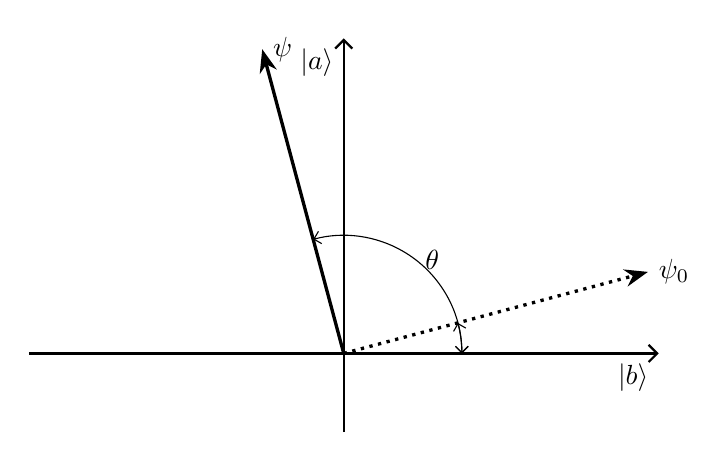
\begin{tikzpicture}[
            > = Straight Barb,
phasor/.style = {very thick,-{Stealth}},
angles/.style = {draw, <->, angle eccentricity=1,
                 right, angle radius=15mm}
                        ]
% coordinates
    \draw[->, thick] (-4,0) -- (4,0) coordinate (x) node[below left] {$\ket{b}$};
    \draw[->, thick] (0,-1) -- (0,4) node[below left] (y) {$\ket{a}$};
% phasors
    \draw[phasor, dotted] (0,0) -- (15:4) coordinate (i)  node[right] {$\psi_0$};% used polar coordinates
    \draw[phasor] (0,0) -- (105:4) coordinate (k)  node[right] {$\psi$};% used polar coordinates
% angles drawn by pic
\coordinate (X)   at (0,0);
\draw
    pic["",angles] {angle=x--X--i}
    pic["$\theta$",angles] {angle=x--X--k}
;
\end{tikzpicture}

So exceeding one query does not make much difference, but when we do this a few number of times, $\psi$ keeps on deviating from the required state. And then after some number of such iterations, it again starts to return to the position. And this "some number of iterations" is less than $\sqrt{N}$ because since the angle made from $\ket{b}$ is large, the iterations of the algorithm make huge changes in the states and thus requires fewer steps.

\textbf{Note - This was observed when there was only one desirable state. With multiple desirable states a similar pattern was followed but not accurately.}

\subsection{Assumption about the given black box}
It is assumed that a quantum circuit has already been implemented that identifies the answer that we use as a black box. Well, if such a black box has been implemented, the maker of the black box would already know about the desired state.\\
I think that maybe in future a situation may arise when the implemented black box is provided by nature and the algorithm may be used to find the desirable state.\\
But nevertheless, this amazing algorithm does given an idea about the power of Quantum Computing.

\end{document}.
